\documentclass[12pt]{book}
\usepackage[margin=.85in]{geometry} % for MARGIN
\usepackage[many]{tcolorbox}    	% for COLORED BOXES (tikz and xcolor included)

\usepackage{multirow}
\usepackage{tabularx}
\usepackage{multicol}   
\usepackage{enumerate}
\usepackage[shortlabels]{enumitem}
\usepackage{varwidth}
\usepackage{tasks}
\usepackage[export]{adjustbox}
\usepackage{array} % For m{} column type

\usepackage{titleps}
\usepackage{setspace}               % for LINE SPACING
\usepackage[⟨options⟩]{fancyhdr}
\usepackage{enumitem}
\setlist{nosep}
\usepackage{tikz}
\usepackage{pgfplots}
\pgfplotsset{compat=1.5.1}
\usetikzlibrary{datavisualization}
\usetikzlibrary{datavisualization.formats.functions}

\newcommand{\D}{\displaystyle}


\setlength\parindent{0pt}   % killing indentation for all the text
\setstretch{1.3}            % setting line spacing to 1.3
\setlength\columnsep{0.25in} % setting length of column separator
\pagestyle{fancy}           % setting pagestyle to be headings

\usepackage[]{titlesec}

\fancyhead[L]{Math V04 - College Algebra}
\fancyhead[R]{Christina Papazacharioudakis}

\tcbset{
    sharp corners,
    colback = white,
    before skip = 0.2cm,    % add extra space before the box
    after skip = 0.5cm      % add extra space after the box
}                           % setting global options for tcolorbox

    \newtcolorbox{boxR}{
    fontupper = \color{black}, % font color
    boxrule = 1.5pt,
    colframe = black,
    rounded corners,
    arc = 5pt   % corners roundness
}



\begin{document}


{\large \textbf{5.2 Power Functions and Polynomial Functions}}

In the previous section, we looked at studying the graphs of a quadratic function,
$$f(x)=ax^2+bx+c$$
Now, we will expand our understanding of a broader category of functions called \textbf{power functions} and \textbf{polynomial functions}. 

\begin{boxR}
\textbf{Power Function}
    \vspace{1mm}
    \hline
    \vspace{2mm}
A power function is a function that can be represented in the form 
    $$ f(x) = ax^n$$
where $a$ and $n$ are real numbers. $a$ is called the \textbf{coefficient}. $x$ is the \textbf{variable}, and $n$ is the \textbf{exponent} of the variable.
\end{boxR}

\underline{\textbf{Example 1 - Determine the Variable, Exponent, and Coefficient in a Power Function}}
Determine the Variable, Exponent, and Coefficient in the following Power Functions. 

\begin{multicols}{3}
\begin{enumerate}[(a)]
    \item $\D f(x)=\frac{1}{3}x^2$
    \item $\D g(t)= 2t^{\frac{5}{3}}$
    \item $\D f(x)=x^2$
\end{enumerate}
\end{multicols}
\vspace{30mm}
\begin{multicols}{3}
\begin{enumerate}[label=(\alph*),start=5]
    \item $\D f(x)=x^{\frac{1}{2}}$
    \item $\D g(t)=3t^{-2}$
\end{enumerate}
\end{multicols}
\vspace{30mm}


\textbf{Question:} Is $\D f(x) = 2^x$ a power function?
\newpage

{\large \textbf{Identifying the End Behavior of Power Functions}}

The picture below shows the graphs of $f(x)=x^2$, $g(x)=x^4$, and $h(x)=x^6$. 

\centerline{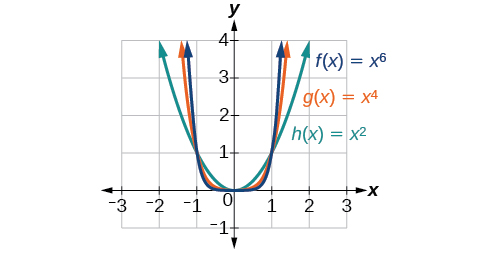
\includegraphics[scale=1.4]{Chapter 5/5.2-figure1.jpeg}}


Notice these graphs have a very similar shape to the toolkit function $f(x)=x^2$. As the powers increase (even powers), the graph ``flattens" near the origin and then becomes steeper moving away from the origin.

\bigskip

As $x$ gets very large, what happens to $f(x), g(x), \text{ and}$ $h(x)$?
\vspace{30mm}

As $x$ gets very small, what happens to $f(x), g(x), \text{ and}$ $h(x)$?
\vspace{30mm}


\newpage

More formally in math, to describe the behavior as numbers become larger and larger (or smaller and smaller), we use the idea of infinity with arrows. Looking at $f(x)$ again, we can say: 

\vspace{40mm}

\begin{boxR}
\textbf{Arrow Notation}
\vspace{1mm}
\hline
\vspace{2mm}
     When $x$ gets really large, we write:  $x \to \infty$ \\
     When $x$ gets really small, we write:  $x \to -\infty$ \\
     If $f(x)$ gets really large ($y$-values), we write: $f(x) \to \infty$ \\
    If $f(x)$ gets really small ($y$-values), we write: $f(x) \to -\infty$
    \bigskip
    
    The arrow ($\to$) means ``goes to"
\end{boxR}

Below is the graph of $f(x)=x^3$, $g(x)=x^5$, $h(x)=x^7$.
\bigskip 

\centerline{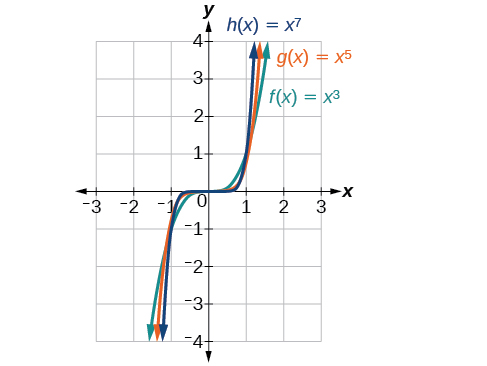
\includegraphics[scale=1.3]{Chapter 5/5.2-figure2.jpeg}}


Notice these graphs have a very similar shape to the toolkit function $f(x)=x^3$. As the powers increase (odd powers), the graph “flattens” near the origin and then becomes steeper moving away from the origin.


\newpage

\underline{\textbf{Example 2 - Use Arrow Notation to Describe the End Behavior of a Graph}}

Use arrow notation to describe the behavior of $f(x)=x^3$, $g(x)=x^5$, $h(x)=x^7$.

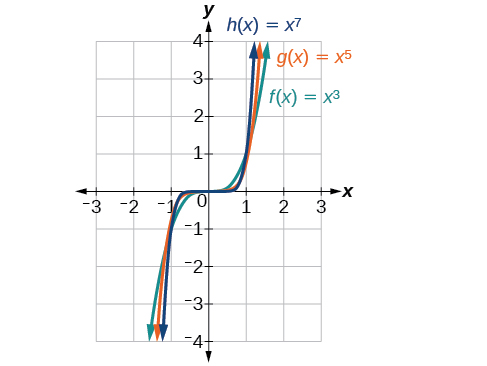
\includegraphics[scale=1.1]{Chapter 5/5.2-figure2.jpeg}


\newpage

The behavior of the graph of a function is referred to as the \textbf{end behavior} when the input values get very large ($x \to \infty$) and get very small ($x \to -\infty)$.
\bigskip



\begin{center}
\begin{tabular}{|c|c|c|}
\hline
\multicolumn{3}{|c|}{End Behavior for $f(x)=ax^n$ ($n$ is a positive integer)} \\
 \hline
 Sign of Coefficient &  If $n$ is an Even Power  & If $n$ is an Odd Power \\ 
 \hline $a>0$
&  \begin{tikzpicture}[scale=.5, transform shape]
\begin{axis}[
    ymin=-3,
    ymax=3,
    xmin=-3,
    xmax=3,
    axis on top=true,
    axis x line=middle,
    axis y line=middle,
    axis line style={latex-latex},
    xlabel=$x$,
    ylabel=$y$,
%    xtick distance=1,
%    ytick distance=10,
  %   axis equal = true, 
    every axis x label/.style={at={(ticklabel* cs:1.0)}, anchor=west,},
    every axis y label/.style={at={(ticklabel* cs:1.0)}, anchor=south,}
]
    \pgfplotsset{ticks=none}
   % \draw(axis cs:0,0) circle[very thick, blue, radius=1];
    \addplot [<->][domain=-1.3:1.3, very thick, samples=100, blue] {x^4};
\end{axis}
\end{tikzpicture}
& 
\begin{tikzpicture}[scale=.5, transform shape]
\begin{axis}[
    ymin=-3,
    ymax=3,
    xmin=-3,
    xmax=3,
    axis on top=true,
    axis x line=middle,
    axis y line=middle,
    axis line style={latex-latex},
    xlabel=$x$,
    ylabel=$y$,
%    xtick distance=1,
%    ytick distance=10,
  %   axis equal = true, 
    every axis x label/.style={at={(ticklabel* cs:1.0)}, anchor=west,},
    every axis y label/.style={at={(ticklabel* cs:1.0)}, anchor=south,}
]
    \pgfplotsset{ticks=none}
   % \draw(axis cs:0,0) circle[very thick, blue, radius=1];
    \addplot [<->][domain=-1.25:1.25, very thick, samples=100, blue] {x^5};
\end{axis}
\end{tikzpicture}
\\
& As $x \to \infty$, $f(x) \to \infty$ & As $x \to \infty$, $f(x) \to \infty$ \\ 
& As $x \to -\infty$, $f(x) \to \infty$ &  As $x \to -\infty$, $f(x) \to -\infty$ \\

 \hline 
 $a<0$

&  \begin{tikzpicture}[scale=.5, transform shape]
\begin{axis}[
    ymin=-3,
    ymax=3,
    xmin=-3,
    xmax=3,
    axis on top=true,
    axis x line=middle,
    axis y line=middle,
    axis line style={latex-latex},
    xlabel=$x$,
    ylabel=$y$,
%    xtick distance=1,
%    ytick distance=10,
  %   axis equal = true, 
    every axis x label/.style={at={(ticklabel* cs:1.0)}, anchor=west,},
    every axis y label/.style={at={(ticklabel* cs:1.0)}, anchor=south,}
]
    \pgfplotsset{ticks=none}
   % \draw(axis cs:0,0) circle[very thick, blue, radius=1];
    \addplot [<->][domain=-1.3:1.3, very thick, samples=100, blue] {-x^4};
\end{axis}
\end{tikzpicture}
& 
\begin{tikzpicture}[scale=.5, transform shape]
\begin{axis}[
    ymin=-3,
    ymax=3,
    xmin=-3,
    xmax=3,
    axis on top=true,
    axis x line=middle,
    axis y line=middle,
    axis line style={latex-latex},
    xlabel=$x$,
    ylabel=$y$,
%    xtick distance=1,
%    ytick distance=10,
  %   axis equal = true, 
    every axis x label/.style={at={(ticklabel* cs:1.0)}, anchor=west,},
    every axis y label/.style={at={(ticklabel* cs:1.0)}, anchor=south,}
]
    \pgfplotsset{ticks=none}
   % \draw(axis cs:0,0) circle[very thick, blue, radius=1];
    \addplot [<->][domain=-1.25:1.25, very thick, samples=100, blue] {-x^5};
\end{axis}
\end{tikzpicture}
\\
& As $x \to \infty$, $f(x) \to -\infty$ & As $x \to \infty$, $f(x) \to -\infty$ \\ 
& As $x \to -\infty$, $f(x) \to \infty$ &  As $x \to -\infty$, $f(x) \to \infty$ \\
\hline
\end{tabular}
\end{center}

\underline{\textbf{Example 3 - Identify the End Behavior of a Power Function}}

Describe the end behavior of the graph of $f(x)=x^8$.


\newpage

\begin{boxR}
    \textbf{How To}
    \vspace{1mm}
    \hline
    \vspace{2mm}
    Given a power function $f(x)=ax^n$ ($n$ is a positive, whole number), identify the end behavior. 
    \begin{enumerate}
        \item Determine whether the power is even or odd.
        \item Determine whether the coefficient is positive or negative.
        \item Reference table above.
    \end{enumerate}
\end{boxR}


\underline{\textbf{Example 4 - Identify the End Behavior of a Power Function}}

Describe the end behavior of the graph of $f(x)=-x^9$.


\newpage
{\large \textbf{Identifying End Behavior of Polynomial Functions}}
    
Recall from Chapter 1 (our first day of class!!) we talked about polynomials.

\begin{boxR}
   \textbf{Polynomial Functions}
   \vspace{1mm}
   \hline
   \vspace{2mm}
   Let $n$ be a non-negative integer. A \textbf{polynomial function} is a function that can be written in the form
   $$ f(x)=a_nx^n + a_{n-1}x^{n-1}+ \ldots + a_2x^2 + a_1x +a_0$$
   Each $a_i$ is a coefficient. Each expression $a_ix^i$ is the term.
\end{boxR}

\centerline{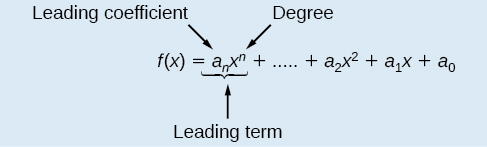
\includegraphics[scale=1]{Chapter 5/5.2-figure4.jpeg}}

\bigskip
\underline{\textbf{Example 5 - Identifying the Degree and Leading Coefficient of a Polynomial Function}}

Identify the degree, leading term, and leading coefficient of the following polynomial functions. 
\begin{enumerate}[(a)]
    \item $f(x)= -4x^3+2x^2+3$
    \vspace{30mm}
    \item $g(t)= -t^3+6t-2$
\end{enumerate}

\newpage

{\large \textbf{Identifying End Behavior of Polynomial Functions}}

To determine the end behavior of a polynomial, we look at its leading term. The end behavior of the polynomial will match the end behavior of the leading term, which is a power function.
\vspace{3mm}


\begin{center}
\renewcommand{\arraystretch}{1.7} % Adjust row height for better vertical alignment
\begin{tabular}{|m{5cm}|m{4cm}|m{7cm}|}
\hline
\multicolumn{3}{|c|}{End Behavior of a Polynomial} \\
\hline
Polynomial Function & Leading Term & Graph of Polynomial \\
\hline
$f(x) = 5x^4+2x^3-x-4$ &  & 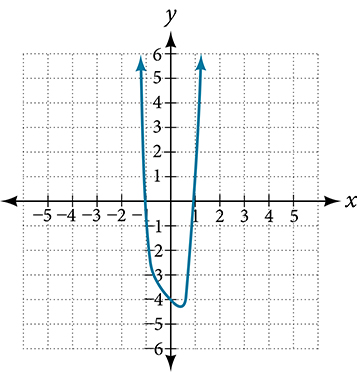
\includegraphics[scale=.5]{Chapter 5/5.2-figure5.jpeg} \\
 &  &  \\
\hline
$f(x)=-2x^6-x^5+3x^4+x^3$ & & 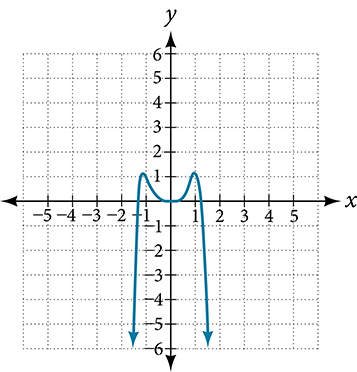
\includegraphics[scale=.5]{Chapter 5/5.2-figure6.jpeg} \\
&  &  \\
\hline
\end{tabular}
\end{center}

\newpage

\begin{center}
\renewcommand{\arraystretch}{1.8} % Adjust row height for better vertical alignment
\begin{tabular}{|m{5cm}|m{4cm}|m{7cm}|}
\hline
Polynomial Function & Leading Term & Graph of Polynomial \\
\hline
$f(x) = 3x^5-4x^4+2x^2+1$ &  & 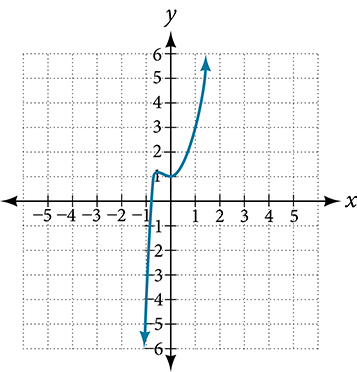
\includegraphics[scale=.5]{Chapter 5/5.2-figure7.jpeg} \\
 &  &  \\
\hline
$f(x)=-2x^6-x^5+3x^4+x^3$ & & 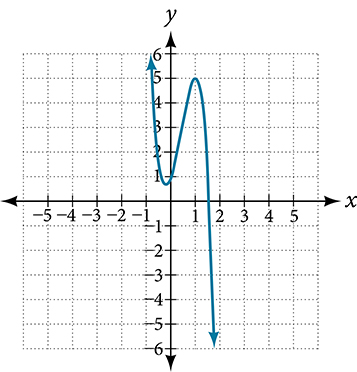
\includegraphics[scale=.5]{Chapter 5/5.2-figure8.jpeg} \\
&  &  \\
\hline
\end{tabular}
\end{center}


\newpage

















\newpage

\underline{\textbf{Example 6 - Determine the End Behavior of a Polynomial}}

Determine the end behavior of the polynomial function, $f(x)=-3x^4-9x^3+12x^2$.

\vspace{50mm}

{\large \textbf{Identifying Local Behavior of Polynomial Functions}}

Now that we looked at the end behavior of a polynomial, we now focus on what is happening in the ``middle" of the polynomial. So what could possibly happen in the middle?  and where the behavior changes. A \textbf{turning point} is a point at which the function changes from increasing to decreasing, or decreasing to increasing. Notice that we also have is $x$ and $y$ intercepts in the ``middle".
\bigskip

\centerline{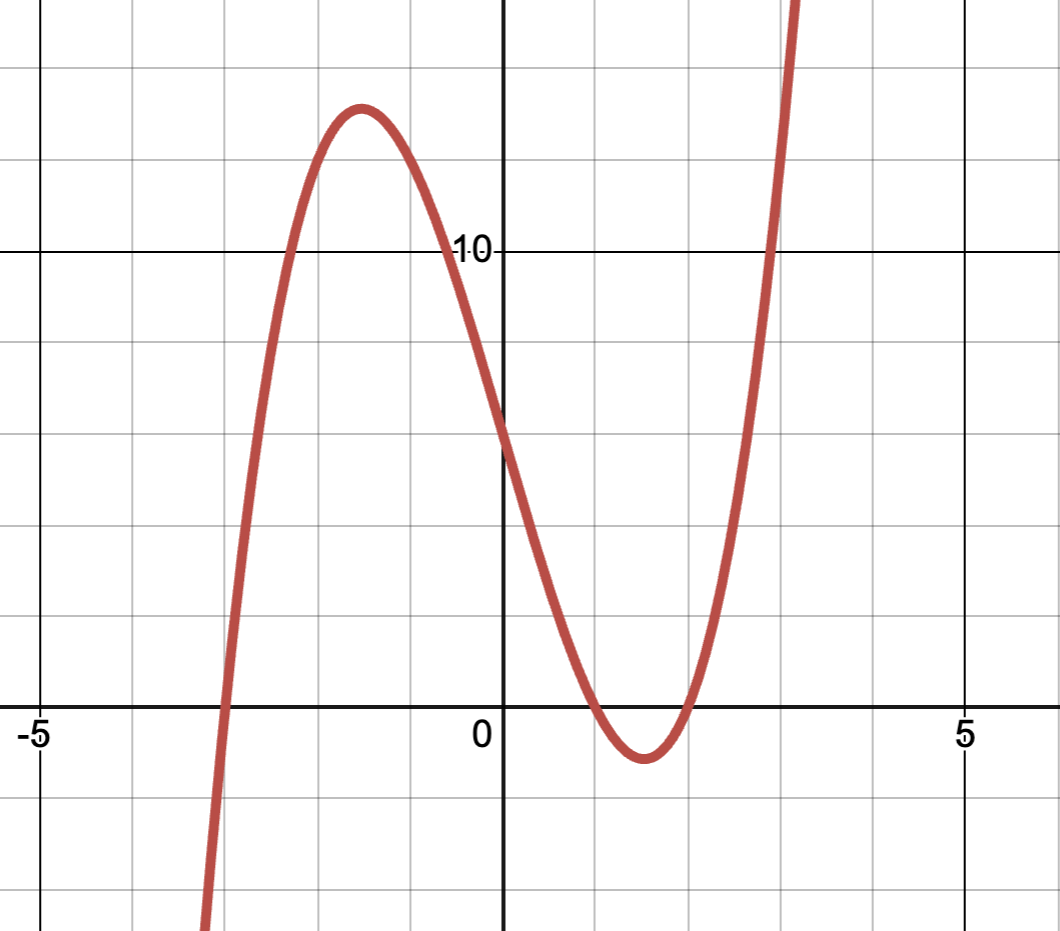
\includegraphics[scale=.4]{Chapter 5/5.2-figure9.png}}




\newpage

\underline{\textbf{Example 7 - Determining the Intercepts of a Polynomial Function}}

Given the polynomial function  $f(x)=(x-2)(x+1)(x-4)$, determine the intercepts. Then look at the end behavior of $f(x)$. Use information about the intercepts and end behavior to determine how many turning points the graph has. 

\vspace{150mm}

\begin{boxR}
  \textbf{Intercepts and Turning Points of Polynomials}
  \vspace{1mm}
  \hline
  \vspace{2mm}
  A polynomial of degree $n$ will have, at most, $n$  $x$-intercepts and at most, $n-1$ turning points.
\end{boxR}
\newpage


\underline{\textbf{Example 8 - Determine the Number of Intercepts and Turning Points of a Polynomial}}

Without graphing the function, determine the local behavior of the function by finding the maximum number of $x$-intercepts and  maximum number of turning points for $$f(x)=-3x^{10}+4x^7-x^4+2x^3$$.

\vspace{30mm}

\underline{\textbf{Example 9 - Determine the Number of Intercepts and Turning Points with a Graph}}
What can we conclude about the degree of the polynomial represented by the graph below?
\centerline{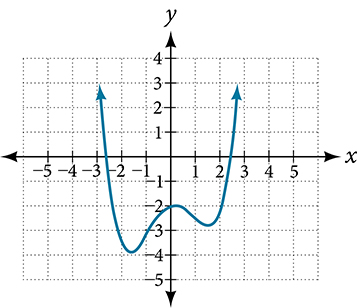
\includegraphics[scale=.6]{Chapter 5/5.2-figure10.jpeg}}


\vspace{50mm}
In the next section, we will build more on how to find the exact amount of turning points and $x$-intercepts.


 




\end{document}


